% 45 minutes including demos of JIT and pkg_composability, exlcluding
% Julia installation.

\documentclass[t]{beamer}
\usepackage{color}
\usepackage{amsmath}
\usepackage{pdfpages}

\definecolor{dkgreen}{rgb}{0,0.5,0}
\definecolor{gray}{rgb}{0.5,0.5,0.5}
\definecolor{Maroon}{rgb}{0.6,0,0}
\newcommand\df{\bf\color{Maroon}}
\newcommand\dff{\bf\color{dkgreen}}
\setbeamercolor{background canvas}{bg=}
%\usetheme{TuringLight}
%\usetheme{TuringDark}

% Presentation data
\title{\color{Maroon} Introduction to Julia}
%\subtitle{\small An introduction}
\date{November, 2021}
\author{Anthony Blaom, with help from Quinn Asena}

% Uncomment any of these lines below to set custom size for each of the font sizes.
% The default value is shown in the comment.
%\setlength{\titlefontsize}{6.875\basefontsize}
%\setlength{\subtitlefontsize}{4.375\basefontsize}
%\setlength{\frametitlesize}{2.625\basefontsize}
%\setlength{\framesubtitlesize}{1.625\basefontsize}
%\setlength{\bodytextsize}{2\basefontsize}
%\setlength{\blocktitlesize}{\bodytextsize}
%\setlength{\blockbodysize}{\bodytextsize}

% Start document
\begin{document}

% Title slide (details filled from presentation data fields above)

% \begin{frame}
%   \frametitle{Installing the tutorials}

%   Please follow instructions at:
%   \begin{center}
%     {\df github.com/ablaom/MachineLearningInJulia2020}
%   \end{center}
% \end{frame}

\begin{frame}
        \titlepage
\end{frame}

\begin{frame}
  \frametitle{Introducing Julia}
  Julia is an open source, general-purpose programming language, in
  the fourth year of its first {\df stable} release 1.0.\pause

  \begin{block}{Key take aways}
    \begin{itemize}
    \item Julia let's you write {\df fast}
      code {\df fast}.\pause
    \item Maximally hackable.
  \end{itemize}
  \end{block}
\end{frame}

% lego analogy
\includepdf[scale=1.3,pages={1,3}]{lego.pdf}


\begin{frame}
  \frametitle{Introducing Julia}
  Julia is an open source, general-purpose programming language, in
  the fourth year of its first {\df stable} release 1.0.

  \begin{block}{Key take aways}
    \begin{itemize}
    \item Julia let's you write {\df fast}
      code {\df fast}.
    \item Maximally hackable.
    \item Julia's design makes {\df extending} Julia code easy,
      promoting a relatively rapid expansion of third party libraries.
    \end{itemize}
  \end{block}
\end{frame}

\begin{frame}
  \frametitle{Julia's secret sauce}
    \begin{itemize}
    \item {\df Just-in-time compilation}
    \item {\df Multiple dispatch}
    \item {\df Abstract type system} (typing is dynamic, nominative and parametric)
  \end{itemize}
\end{frame}

\begin{frame}
  \begin{block}{Workshop resources:}
    {\large\texttt{github.com/ablaom/HelloJulia.jl}}
    \end{block}
\end{frame}

\begin{frame}
  \begin{block}{Secret sauce demo:}
    {\large\texttt{github.com/ablaom/HelloJulia.jl/}}\newline
    {\large\texttt{blob/dev/demos/secret\_sauce/notebook.ipynb}}
    \end{block}
\end{frame}
%
\begin{frame}
  \begin{block}{Package composability demo:}
    {\large\texttt{github.com/ablaom/HelloJulia.jl/}}\newline
    {\large\texttt{blob/dev/demos/pkg\_composability/notebook.ipynb}}
    \end{block}
\end{frame}

\begin{frame}[plain]
  %  \begin{center}
     \includegraphics[scale=0.25]{mandel.png}
%   \end{center}
\end{frame}
% stars
\begin{frame}[plain]
  %  \begin{center}
     \includegraphics[scale=0.30]{julia_stars.png}
%   \end{center}
\end{frame}

% 2018 conference (2021: 3 x talks, 50 x registration):
\includepdf[pages=10]{Sebastian.pdf}

% growth stats 2020 - 2021:
\begin{frame}[plain]
  %  \begin{center}
     \includegraphics[scale=0.70]{julia_stats.png}
%   \end{center}
\end{frame}

% high profile applications:
\includepdf[pages=18-21]{julia_for_ecologists.pdf}
\includepdf[pages=23]{julia_for_ecologists.pdf}

% \begin{frame}
%   \frametitle{The Two Language Problem}
%   \begin{itemize}

% \item   Older programming languages like C and FORTRAN are designed to {\em
%     run} fast. Almost all {\df computationally demanding} tasks
%   (weather forecasting, machine learning, etc) are performed by
%   calling code written in these languages. \pause
  
% \item ``Scripting'' languages like python, MATLAB, and R allow you
%   quickly {\df wrap} computational tasks into {\df customized and easily
%     modified workflows}. They also accelerate {\df testing and
%     protyping} of new computational algorithms.\pause

% \item These languages are {\df too slow} for computationally intensive tasks.
% \end{itemize}
% \end{frame}

\begin{frame}
  \frametitle{Popular libraries (packages)}
  These are all pretty mature:
  \begin{itemize}
  \item DataFrames.jl and CSV.jl  - {\df in-memory data manipulation}
  \item Plots.jl (also easy to call R's ggplot())
  \item $\star$ JuMP.jl - {\df constrained optimization}
  \item $\star$ DifferentialEquations.jl
  \item StatsModels.jl, GLM.jl - {\df traditional stats models}
  \item Flux.jl  - {\df deep learning}
  \item $\star$ Turing.jl, Soss.jl, ... {\df probabilistic programmming}
  \item MLJ.jl - multi-pardigm {\df machine learning} platform
  \item Pluto.jl - {\df ``reactive'' notebooks}
  \end{itemize}
\end{frame}

% lines of code versus mean run time:
\includepdf[pages=11]{julia_for_ecologists.pdf}
  
\begin{frame}
  \frametitle{Why  is two languages a problem ?}
  \begin{itemize}
    \item Can't easily {\df modify} core algorithms
    \item Barrier to {\df understanding algorithms} even if not seeking to modify them
    \item Complicates installation of a complete software stack
    (package {\df dependency hell}, manual interventions)
    \item Barrier to {\df transparency} and {\df reproducibility}
    \item Barrier to {\df composing libraries} (e.g., automatic differentiation)
    \item {\df Hampers innovation}, development of novel algorithms
  \end{itemize}
\end{frame}

% slows innovation engineers <--> researchers 
\includepdf[scale=1.3,pages={1,2,4}]{slows_innovation.pdf}

\begin{frame}[plain]
  \frametitle{Fast code written fast: DifferentialEquations.jl}
  % \frametitle{DifferentialEquations.jl}
  %  \begin{center}
     \includegraphics[scale=0.27]{de_solver_software_comparsion.pdf}
%   \end{center}
\end{frame}

% % data science pipeline
% \includepdf[pages=3-5]{Sebastian.pdf}

% \begin{frame}[plain]
%     \includegraphics[scale=0.45]{benchmarks.png}
% \end{frame}


% \begin{frame}
%   \frametitle{The Expression Problem}
%   As in any kind of architecture, the central concerns of a
%   programming language are {\df form} and {\df function}. Roughly
%   speaking, the {\df Expression Problem} is the problem of how to
%   represent data (form) and how to articulate required behaviour
%   (function) in way that allows {\df extension} of both in an optimal
%   and safe way.\pause
%   \begin{itemize}
%     \item Object oriented languages typically score poorly here (Ruby has a
%       dirty way, Scala a clean workaround).
%     \item Julia scores well. {\df Proof:} \pause Large code-reuse, package composibility
%   \end{itemize}
% \end{frame}


\begin{frame}
  \frametitle{Other features}
  \begin{itemize}
    \item Fast user-defined composite types (C-like structs)
    \item Lisp-like macros/metaprogramming
    \item Call C functions directly
    \item Can wrap Python, R Java/Scala
    \item State-of-the-art distributed computing and multi-threading support
  \end{itemize}
\end{frame}

% code snippet:
\begin{frame}
  \frametitle{Other features (continued)}
  \begin{itemize}
  \item First-class math support
    \item Exellent REPL (console)
    \item Built-in package manager
    \item Automatic differentiation (Zygote.jl)
  \end{itemize}
\end{frame}

\begin{frame}
  \frametitle{Drawbacks}
  For most users all serious drawbacks derive from Julia's young age:
  \begin{itemize}
     \item Smaller number of libraries
     \item Smaller community of users
     \item Some interfaces and tooling less polished
     \item More bugs (in libraries, few in language itself)
  \end{itemize}
  Other drawbacks and annoyances:
  \begin{itemize}
     \item Limited support for exporting programs as stand-alone executables.
     \item Wating for first-time/pre compilation.
  \end{itemize}
\end{frame}

% \begin{frame}
%   \frametitle{The Julia data science ecosystem}
%   \begin{block}{Data manipulation and exploratory data analysis}
%   \begin{itemize}
%       \item DataFrames.jl (stable release)
%       \item Queryverse.jl for querying (in-memory) data sources (stable release)
%       \item Mature plotting packages, including a common front-end Plots.jl for:
%         matplotlib, Plotly, Vega, GR, \& others.  Makie.jl is native julia and
%         runs on a GPU.\pause
%   \end{itemize}
% \end{block}
% \end{frame}
% \begin{frame}
%   \begin{block}{Models}
%   \begin{itemize}
%      \item Wrappers exist for: scikit-learn, XGBoost, LightGBM, SVM (also have MLJ interfaces)\pause
%      \item Julia native libraries for Gradient Tree Boosting, general gradient descent models (neural networks),
%          Clustering, Decision Trees, Random Forests, General Linear Models, Elastic Net \& Lasso, naive bayes,
%          probabilistic programming models, guassian processes, \ldots\pause
%   \end{itemize}
%   \end{block}
%   \begin{block}{ML Frameworks}
%   \begin{itemize}
%      \item MLJ.jl (multi-paradigm)
%      \item MLAutoPipeline.jl (multi-paradigm)
%      \item ScikitLearn.jl (wrapper)
%      \item FastAI.jl (gradient descent)
%   \end{itemize}
%   \end{block}
% \end{frame}

% \begin{frame}
%   \mbox{}
%   \vspace{4\baselineskip}
%   \begin{center}
%     \large {\df MLJ} (Machine Learning in Julia)
%   \end{center}
% \end{frame}

% \begin{frame}
%   \vspace{0\baselineskip}
%   \begin{center}
%     \includegraphics[scale=0.2]{Turing_logo.png}
%     \includegraphics[scale=0.35]{UoA_logo.png}

%     \includegraphics[scale=0.2]{IQVIA_logo.png}
%     \includegraphics[scale=0.12]{NESI-logo.jpg}
%     \includegraphics[scale=0.12]{warwick.png}
%     \includegraphics[scale=0.12]{julia.png}
%   \end{center}
% \end{frame}

% \begin{frame}
%   \frametitle{The Team}

%   {\small
%     {\dff Core design:} A. B., Franz Kiraly, Sebastian Vollmer\\[1\baselineskip]

%     {\dff Lead development:} A. B., Thibaut Lienart \\[1\baselineskip]

%     {\dff Other contributors:} Diego Arenas, Samuel Okon, Yiannis Simillides, Julian Samaroo, Ayush Shridar, Mosè Giordano\ldots \\[1\baselineskip]

%     {\dff Julia language consultants:} Avik Sengupta, Dilum Aluthge\\[1\baselineskip]}

% \end{frame}

% \begin{frame}
%   \frametitle{Contributing}
%   \begin{itemize}
%      \item Star the MLJ.jl repo!
%      \item Report problems by raising issues
%      \item Contribute a tutorial at DataScienceTutorials.jl
%      \item Implement the MLJ interface new models
%      \item 1+ yr Postdoc/Software Engineer position; contact Sebastian
%        at svollmer@turing.ac.uk
%      \end{itemize}
% \end{frame}

% \begin{frame}
%   \frametitle{Interacting}
%    Zoom Webinar provides {\bf two} ways to interact:

%   \begin{block}{Q/A}
%     For asking panelists questions
%   \end{block}

%   \begin{block}{Chat}
%     For discussion {\em not} monitored by panelists
%   \end{block}\pause

%   \begin{block}{\includegraphics[scale=0.1]{raise_hand_forbidden.png}}
%   \end{block}

% \end{frame}

% \begin{frame}
%   \frametitle{Who?}
%   \begin{block}{Prerequisites:}\pause
%     \begin{itemize}
%     \item familiar with machine learning principles
%     \item basic Julia skills
%     \item experience using DataFrames or similar a plus
%     \end{itemize}
%   \end{block}
% \end{frame}

% %% Intro to machine learning process

% \begin{frame}
%   \frametitle{Supervised Learning}
%   Learning to {\df predict} some target variable {\df\large y} from a
%   knowledge of some other variables {\df \large X} (the {\it input features}).\pause
%   \begin{center}
%     \includegraphics[scale=0.17]{X.png}\mbox{~~~~}
%     \includegraphics[scale=0.17]{y.png}
%   \end{center}
% \end{frame}

% \begin{frame}
%   \frametitle{Supervised Learning}
%    \begin{center}
%     \includegraphics[scale=0.6]{overfitting1.png}
%    \end{center}
% \end{frame}

% \begin{frame}
%   \frametitle{Supervised Learning}
%    \begin{center}
%     \includegraphics[scale=0.6]{overfitting2.png}
%    \end{center}
% \end{frame}

% \begin{frame}
%   \frametitle{Supervised Learning}
%    \begin{center}
%     \includegraphics[scale=0.6]{overfitting3.png}
%    \end{center}
% \end{frame}

% \begin{frame}
%   \frametitle{Supervised Learning}
%    \begin{center}
%     \includegraphics[scale=0.6]{overfitting4.png}
%    \end{center}
% \end{frame}

% \begin{frame}
%   \frametitle{Supervised Learning}
%    \begin{center}
%     \includegraphics[scale=0.6]{overfitting5.png}
%    \end{center}
% \end{frame}

% \begin{frame}
%   \frametitle{Supervised Learning}
%    \begin{center}
%     \includegraphics[scale=0.6]{overfitting6.png}
%    \end{center}
% \end{frame}

% \begin{frame}
%   \frametitle{Unsupervised Learning}
%   Learning data {\df transformations}, e.g., dimension reduction
%    \begin{center}
%     \includegraphics[scale=0.13]{PCA.png}
%    \end{center}
% \end{frame}

% \begin{frame}
%   \frametitle{Unsupervised Learning}
%   Learning data {\df transformations}, e.g., dimension reduction
%    \begin{center}
%     \includegraphics[scale=0.13]{PCA2.png}
%    \end{center}
% \end{frame}

% \begin{frame}
%   \frametitle{A plethora of models}
%   \begin{center}
%     \includegraphics[scale=0.08]{packages.jpg}
%   \end{center}
% \end{frame}

% \begin{frame}
%   \frametitle{Data science competitions (kaggle)}
%   \vspace{-1.0\baselineskip}
%     \begin{center}
%       \includegraphics[scale=0.16]{kaggle1.png}
%       \includegraphics[scale=0.16]{kaggle2.png}
%       \includegraphics[scale=0.16]{kaggle3.png}
%   \end{center}
% \end{frame}


% \begin{frame}
%   \frametitle{What?}
%   \begin{block}{What is MLJ?}\pause
%      \begin{itemize}
%      \item A toolbox providing a {\df uniform interface} for {\df
%          fitting}, {\df evaluating}, {\df tuning}, and {\df
%          controlling} a broad variety of machine learning models (not
%        just ``deep learning'' models!)
%           \item Provides common {\df preprocessing tasks} (such as data cleaning
%             and type coercion)
%           \item Allows for model {\df composition} (e.g., pipelining, stacking)
%       \end{itemize}
%     \end{block}
%   \end{frame}

% \begin{frame}
% \frametitle{Toolboxes in other ecosystems}
%   \begin{center}
%     \includegraphics[scale=0.4]{other_toolboxes.png}
%   \end{center}
% \end{frame}

%%%

% \begin{frame}
%   \frametitle{Distinguishing features}
%      \begin{itemize}
%      \item Written in Julia (one language!)\pause
%      \item Over 160 models supported (with help of scikit-learn bootstrap)\pause
%      \item Best-in-class model composition API\pause
%      \item Model registry for automatically matching models to data\pause
%      \item Most meta-algorithms are implemented as model wrappers
%        (e.g., tuning, iterative model control)\pause
%      \item Ontological approach to articulating data requirements
%        (``scientific types'')\pause
%      \item Supports a universal Julia tabular data format (Tables.jl)\pause
%      \item Clean design for handling probabilistic predictions\pause
%      \item Persistent tracking of all classes of categorical variables
%       \end{itemize}
% \end{frame}

% \begin{frame}
%   \frametitle{MLJ Limitations}
%      \begin{itemize}
%      \item Feature-sparse data not fully supported
%      \item Integration with models specific to time series and probabilistic programming
%         relatively immature
%      \item No support for online learning, survival analysis,
%        re-inforcement learning, adversarial learning
%      \item No support for training models on data that does not fit into memory
%      \end{itemize}
% \end{frame}

%%%%


% \begin{frame}
%   \frametitle{Why?}
%   \begin{block}{Why learn the MLJ toolbox?}
%     \begin{itemize}
%     \item {\df One language!}\pause

%       Get under the hood to:
%       \begin{itemize}
%       \item increase understanding
%       \item customize behaviour
%       \item add functionality (e.g., new model interfaces)\pause
%       \end{itemize}
%     \item Start-of-the-art {\df model composition} that plays well with everything else.
%     \end{itemize}
%   \end{block}
% \end{frame}



% \begin{frame}
%   \frametitle{Goals for MLJ}\pause
%   \begin{itemize}
%   \item Want {\df usability}, interoperability,
%        extensibility and reproducibility\pause
%   \item Want avoid common {\df pain-points}:
%     \begin{itemize}
%        \item Identifying all models that solve a given task\pause
%        \item Routine operations requiring a lot of code
% %       \item Passage from data source to algorithm-specific
% %         data format
% %       \item Probabilistic predictions: evaluation, inconsistent representations
% %       \item Limitations of {\df model composition} API \pause --- barrier to innovation!
%     \end{itemize}
% %  \item Hope that project adds some focus to Julia ML development more generally
%   \end{itemize}
% \end{frame}

% \includepdf[scale=1,pages={1}]{MLJ_as_lego.pdf}

% \begin{frame}
%   \frametitle{Workshop Overview}
%   \begin{itemize}

%   \item Recap of supervised and unsupervised learning

%   \item Preview of model composition (stacking)

%   \item Part 1 - {\df Data Representation} + exercises

%   \item Part 2 - {\df Selecting, Training and Evaluating Models} + exercises

%   \item  Break

%   \item Part 3 - {\df Transformers and Pipelines} + exercises

%   \item Part 4 - {\df Tuning hyper-parameters} + exercises

%   \item Part 5 - {\df Advanced model composition} (time permitting)

%   \end{itemize}
% \end{frame}


%\begin{frame}
%   \frametitle{Advanced toolbox features}
%   \begin{block}{We want toolboxes that:}\pause
%     \begin{itemize}

%     \item Combine models in more flexible ways, e.g., ensembling,
%       stacking: pipelines $\rightarrow $ {\df learning
%         networks}.\pause
%     \item Avoid redundancies in retraining a learning network.\pause
%     \item Allow systematic tuning of nested parameters across a network\pause
%     \item Implement tuning as {\df model wrapper}\pause
%     \item Automatically match models to specified {\df tasks}
%   \end{itemize}
%   \end{block}
% \end{frame}

% \begin{frame}
%   \frametitle{Model search and tasks}
%   \vspace{-1.5\baselineskip}
%   \begin{center}
%     \includegraphics[scale=0.38]{model_search1.png}
%   \end{center}
% \end{frame}

% \begin{frame}
%   \frametitle{Model search and tasks}
%     \includegraphics[scale=0.30]{Sboston.png}
% \end{frame}

% \begin{frame}
%   \frametitle{Quick performance evaluation}
%   \includegraphics[scale=0.30]{Stree.png}
% \end{frame}

% \begin{frame}
%   \frametitle{Quick performance evaluation}
%   \includegraphics[scale=0.30]{Stree2.png}
% \end{frame}

% \begin{frame}
%   \frametitle{Meta-algorithms as model wrappers}
%   \includegraphics[scale=0.30]{Sforest.png}
% \end{frame}

% \begin{frame}
%   \frametitle{Meta-algorithms as model wrappers}
%   \includegraphics[scale=0.30]{Sforest2.png}
% \end{frame}

% \begin{frame}
%   \frametitle{Meta-algorithms as model wrappers}
%   \includegraphics[scale=0.30]{Sforest3.png}
% \end{frame}

% \begin{frame}
%   \frametitle{Goals for MLJ}
%   \begin{itemize}
%   \item Want {\df usability}, interoperability,
%        extensibility and reproducibility
%   \item Want avoid common {\df pain-points}:
%     \begin{itemize}
%        \item Identifying all models that solve a given task
%        \item Routine operations requiring a lot of code\pause
%        \item Passage from data source to algorithm-specific
%          data format
% %       \item Probabilistic predictions: evaluation, inconsistent representations
% %       \item Limitations of {\df model composition} API \pause --- barrier to innovation!
%     \end{itemize}
% %  \item Hope that project adds some focus to Julia ML development more generally
%   \end{itemize}
% \end{frame}

% \begin{frame}
%   \frametitle{Use any tabular data format}
%   \vspace{-\baselineskip}
%   \begin{center}
%      \includegraphics[scale=0.25]{tableswordcloud.png}
%   \end{center}
% \end{frame}

% \begin{frame}
%   \frametitle{Scientific types}
%   \vspace{-0.5\baselineskip}
%   \begin{center}
%     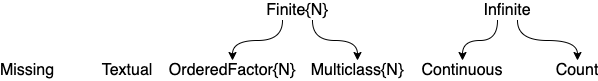
\includegraphics[scale=0.4]{scitypes.png}
%   \end{center}%\pause
% %  {\df Require:} Each julia object can represent only one scientific type
% \end{frame}

% \begin{frame}
%   \frametitle{Categorical data}
%   {\Large categorical $\ne$  integer}\pause
%     \begin{equation*}
%       \mathrm{data} = [1, 2, 2, 2, 1, 2, 1, 1, 3, 2]
%     \end{equation*}
%     \begin{equation*}
%       \mathrm{train} = [1, 2, 2, 2, 1] \quad \mathrm{eval} = [1, 3, 2]
%     \end{equation*}\pause
%     \mbox{}\newline
%     MLJ expects {\tt CategoricalArray.CategoricalValue} for categoricals.
% \end{frame}

% \begin{frame}
%   \frametitle{Probabilistic predictors}
% {\small
% \begin{table}[]
% \centering
% \caption{Conventions for representing probabilistic predictions}
% \label{tab:my-table}
% \begin{tabular}{lll}
% {\df model} & {\df representation} & {\df drawbacks} \\
% binary classifier & single probability & Must specify "true" class  \\
% N-class classifier & N probabilities & \begin{tabular}[c]{@{}l@{}}Inconsistent with binary; \\ must specify class order\end{tabular}  \\
% Gaussian GLM & mean, std & Or should it by mean, var?  \\
% multivariate multiclass & multiple possibilities & No clear convention  \\
% Bayesian model & distribution/sampler object & \begin{tabular}[c]{@{}l@{}}Inconsistent with \\ all of the above\end{tabular}
% \end{tabular}
% \end{table}}
% \end{frame}
% \begin{frame}[plain]
%   \frametitle{Common shortcomings of composition design}
% \begin{itemize}
% \item Composite models do not inherit all the behavior of ordinary
%   models.\pause
% \item Composition limited to non-branching pipelines\pause
% \item Only static (unlearned) target transformations / inverse
%   transformations are supported.\label{four}\pause
% \item Hyper-parameters in homogeneous model ensembles cannot be coupled.\pause
% \item Some sophisticated inhomogeneous ensembling, such as stacking
%   cannot be implemented\pause
% \item Composite models cannot implement multiple operations, for example,
%   both a `predict' and `transform' method.\pause
% \item Nested hyper-parameters or learned parameters not easily accessed.
% \end{itemize}
% \end{frame}

% \begin{frame}
%   \frametitle{Model composition (aka pipelining)}
%   \vspace{1.5\baselineskip}
%     \begin{center}
%     \includegraphics[scale=0.55]{pipeline.png}
%   \end{center}
% \end{frame}

% \begin{frame}
%   \frametitle{Model composition (aka pipelining)}
%   \vspace{1.5\baselineskip}
%     \begin{center}
%     \includegraphics[scale=0.55]{composite.png}
%   \end{center}
% \end{frame}

% \begin{frame}
%   \frametitle{Compact syntax for linear pipeline}
%   \vspace{2\baselineskip}
%     \includegraphics[scale=0.55]{S14.png}

%     \pause Does not generalize!
% \end{frame}

% \begin{frame}
%   \frametitle{The dimension reducer}
%     \begin{center}
%     \includegraphics[scale=0.35]{dim_reducer.png}\\
%   \end{center}
%   \begin{center}
%     \includegraphics[scale=0.32]{S2.png}
%   \end{center}
% \end{frame}

% \begin{frame}
%   \frametitle{The classifier}
%     \begin{center}
%     \includegraphics[scale=0.35]{classifier.png}\\
%   \end{center}
%   \begin{center}
%     \includegraphics[scale=0.32]{S3.png}
%   \end{center}
% \end{frame}

% \begin{frame}
%   \frametitle{Summary of unstreamlined workflow}
%   \vspace{2.5\baselineskip}
%     \begin{center}
%     \includegraphics[scale=0.32]{S4.png}
%   \end{center}
% \end{frame}

% \begin{frame}
%   \frametitle{Refactoring as {\df learning network}: Step 1}
%     \begin{center}
%     \includegraphics[scale=0.32]{S5.png}
%   \end{center}
% \end{frame}

% \begin{frame}
%   \frametitle{Refactoring as {\df learning network}: Step 2}
%   \vspace{-0.4\baselineskip}
%     \begin{center}
%     \includegraphics[scale=0.32]{S6.png}
%   \end{center}
% \end{frame}

% \begin{frame}
%   \frametitle{{\df Training} a learning network}
%     \begin{center}
%     \includegraphics[scale=0.32]{S7.png}
%   \end{center}
% \end{frame}

% % \begin{frame}
% %   \frametitle{{\df Prediction} in a learning network}
% %     \begin{center}
% %     \includegraphics[scale=0.32]{S8.png}
% %   \end{center}
% % \end{frame}

% \begin{frame}
%   \frametitle{{\df Prediction} in a learning network}
%     \begin{center}
%     \includegraphics[scale=0.32]{S11.png}
%   \end{center}
% \end{frame}

% \begin{frame}
%   \frametitle{Summarizing}
%   \vspace{1.5\baselineskip}
%     \begin{center}
%     \includegraphics[scale=0.40]{separate.png}
%   \end{center}
% \end{frame}

% \begin{frame}
%   \frametitle{Summarizing}
%   \vspace{1.5\baselineskip}
%     \begin{center}
%     \includegraphics[scale=0.55]{pipeline.png}
%   \end{center}
% \end{frame}

% \begin{frame}
%   \frametitle{Still a need stand-alone model!}
%   \vspace{1.5\baselineskip}
%     \begin{center}
%     \includegraphics[scale=0.55]{composite.png}
%   \end{center}
% \end{frame}

% \begin{frame}
%   \frametitle{Macro ``exports'' learning network as standalone model}
%     \begin{center}
%     \includegraphics[scale=0.28]{S9.png}
%   \end{center}
% \end{frame}

% % \begin{frame}
% %   \frametitle{Composite is now a model like any other}
% %     \begin{center}
% %     \includegraphics[scale=0.28]{S13.png}
% %   \end{center}
% % \end{frame}

% \begin{frame}
%   \frametitle{Stacking in python}
%   \vspace{-\baselineskip}
%   \begin{center}
%     \includegraphics[scale=0.6]{vecstack.png}
%   \end{center}
% \end{frame}

% \begin{frame}[plain]
%   \frametitle{Stacking in MLJ}
%   \vspace{-\baselineskip}
%   \begin{center}
%     \includegraphics[scale=0.2]{mlj_stack.png}
%   \end{center}
% \end{frame}

% \begin{frame}
%   \frametitle{Goals for MLJ}
%   \begin{itemize}
%   \item Want {\df usability}, interoperability,
%        extensibility and reproducibility
%   \item Want avoid common {\df pain-points}:
%     \begin{itemize}
%        \item Identifying all models that solve a given task
%        \item Routine operations requiring a lot of code
%        \item Passage from data source to algorithm-specific
%          data format\pause
%        \item Probabilistic predictions (evaluation, inconsistent representations, \ldots)
% %       \item Limitations of {\df model composition} API \pause --- barrier to innovation!
%     \end{itemize}
% %  \item Hope that project adds some focus to Julia ML development more generally
%   \end{itemize}
% \end{frame}

% % \begin{frame}
% %   \frametitle{Probabilistic predictors}
% %   In MLJ a probabilistic prediction is a Distributions.Sampler
% %   object, if possible a Distribution.{\df Distribution} object (typical case)
% % \end{frame}

% \begin{frame}
%   \frametitle{Goals for MLJ}
%   \begin{itemize}
%   \item Want {\df usability}, interoperability,
%        extensibility and reproducibility
%   \item Want avoid common {\df pain-points}:
%     \begin{itemize}
%        \item Identifying all models that solve a given task
%        \item Routine operations requiring a lot of code
%        \item Passage from data source to algorithm-specific
%          data format
%        \item Probabilistic predictions: evaluation, inconsistent representations
%        \item Limitations of {\df model composition} API \pause --- barrier to innovation!
%     \end{itemize}
% %  \item Hope that project adds some focus to Julia ML development more generally
%   \end{itemize}
% \end{frame}


% \begin{frame}
%   \frametitle{Road map}\pause
%   \begin{block}{Enhancing functionality: Adding models}
%     \begin{itemize}
%        \item Wrap the scit-learn (python/C) models (Z.~Nugent, D.~Arenas)
%        \item {\df Flux.jl} deep learning (A.~Shridhar)
%        \item {\df Turing.jl} probabilistic programming (M.~Trapp)
%        \item {\df Geostats.jl} (J.~Hoffimann)
%        \item Data cleaning? Feature engineering (featuretools?)\pause
%     \end{itemize}
%   \end{block}
% \end{frame}

% \begin{frame}
%   \frametitle{Road map}
%   \begin{block}{Enhancing core functionality}
%     \begin{itemize}
%     \item Systematic benchmarking
%     \item More comprehensive performance evaluation
%     \item Tuning using Bayesian optimization
%     \item Tuning using gradient descent and AD
%     \item Iterative model control
%   \end{itemize}
%   \end{block}
% \end{frame}

% \begin{frame}
%   \frametitle{Road map}
%   \begin{block}{Broadening scope}
%     \begin{itemize}
%        \item Extend or supplement LossFunctions.jl
%        \item Add sparse data support (NLP)
%        \item Time series
%     \end{itemize}
%   \end{block}
% \end{frame}

% \begin{frame}
%   \frametitle{Road map}
%   \begin{block}{Scalability}
%     \begin{itemize}
%      \item Online learning support and distributed data
%      \item DAG scheduling (J.~Samaroo)
%      \item Automated estimates of cpu/memory requirements
%     \end{itemize}
%   \end{block}
% \end{frame}

% \begin{frame}
%   \vspace{2\baselineskip}
%   \begin{center}
%     {github.com/alan-turing-institute/{\df \Large MLJ.jl}}\\[0.5\baselineskip]
%   {\df Resources for this talk}:  examples/JuliaCon2019/
%   \end{center}
%   \hfill

%   {\tiny
%     {\dff\tiny Core design:} Anthony Blaom, Franz Kiraly, Sebastian Vollmer\\[1\baselineskip]

%     {\dff\tiny Lead contributor:} Anthony Blaom\\[1\baselineskip]

%     {\dff\tiny Julia language consultants:} Mike Innes, Avik Sengupta\\[1\baselineskip]

%     {\dff\tiny Other contributors, past and present:} Dilum Aluthge, Diego
%     Arenas, Edoardo Barp, Gergö Bohner, Michael K. Borregaard,
%     Valentin Churavy, Harvey Devereux, Mosè Giordano, Thibaut Lienart,
%     Mohammed Nook, Piotr Oleśkiewicz, Julian Samaroo, Ayush Shridar,
%     Yiannis Simillides, Annika Stechemesser
%     }


% \end{frame}




% \begin{frame}
%         \finalpage
% \end{frame}

\end{document}

%%% Local Variables:
%%% mode: latex
%%% TeX-master: t
%%% End:
